% !TEX encoding = UTF-8
% !TEX TS-program = pdflatex
% !TEX root = ../tesi.tex

%**************************************************************
\chapter{Analisi dei Requisiti}
\label{cap:analisi_requisiti}
%**************************************************************
Durante il primo periodo di tirocinio è stata svolta la fase di Analisi dei Requisiti, necessaria alla comprensione del dominio e al soddisfacimento della richiesta. Inizialmente è stato effettuato un incontro con il tutor aziendale con il quale sono stati rilevati i requisti obbligatori richiesti dall'azienda da cui è stato possibile identificare un insieme di funzionalità necessarie alla Skill. Successivamente è stato realizzato il documento contenente tutti gli studi di analisi che hanno favorito una buona e corretta progettazione del prodotto. Dalla raccolta dei dati e dalle analisi fatte è stata elaborata una visione ad alto livello del sistema e dei rispettivi casi d’uso. Sono stati inoltre identificati quei punti critici in grado di determinare, in larga misura, la forma finale del prodotto.
La fase di analisi si è infine conclusa con lo studio della VUI (Voice User Interface), e della GUI (Graphical User Interface), che caratterizzano l'esperienza d'uso del prodotto finale. 

%**************************************************************
\section{Obbiettivo}
L’obiettivo del progetto di stage è la realizzazione di una Skill per l’assistente vocale Alexa che sia in grado di accogliere clienti, postini e corrieri all'ingresso degli uffici e notificare in maniera automatica la persona interessata nell'arrivo del visitatore. La Skill è concepita per essere installata sui dispositivi in commercio da Amazon, in particolare sul dispositivo Echo Show 2018. L’obiettivo è quindi quello di realizzare un concierge virtuale che accolga il visitatore e riceva da esso informazioni per mezzo di una conversazione e l’uso di messaggi attraverso lo schermo touch integrato nel dispositivo. Infine tali dati elaborati dai processi di controllo per inviare notifiche al personale.

\subsection{Cliente finale}
Il cliente finale a cui è destinato il prodotto è l’azienda Crispy Bacon Srl, la quale necessita, per ovvi motivi, di un sistema automatizzato che svolga il ruolo di Concierge all'entrata degli uffici. L'azienda intende utilizzare il prodotto come Proof of Concept rappresentativa delle potenzialità delle interfacce conversazionali da utilizzare nelle fasi di proposizione di vendita ai clienti, nonché dopo ulteriori fasi di sviluppo come prodotto finito da vendere nella modalità Software as a Service.

\section{Utenti coinvolti}
Dall'analisi fatta sono emersi i seguenti attori, intesi come persone coinvolte nell'utilizzo della Skill:
\begin{itemize}
    \item Visitatore
        \begin{itemize}
            \item Persona avente appuntamento
            \item Persona non avente appuntamento
            \item Postino
            \item Corriere
        \end{itemize}
    \item Personale di Crispy Bacon
\end{itemize}

\section{Requisiti richiesti}
\label{requisti-richiesti}
I requisiti emersi e richiesti dall'azienda sono stati elaborati e analizzati. Tali requisiti sono interpretabili in tre diversi modi, tutti con il presupposto che questi siano in qualche modo una necessità.
\begin{itemize}
    \item Requisito utente: dal punto di vista dell'utente, è una capacità necessaria per risolvere un problema o raggiungere un obbiettivo;
    \item Requisito software: dal punto di vista della soluzione, è una capacità che deve essere posseduta dal sistema per adempiere all'obiettivo;
    \item Dal punto di vista della documentazione, come una descrizione documentata di una capacità interpretata come un requisito utente o software.
\end{itemize}
\subsection{Identificazione dei Requisiti}
\label{indentificazione-requisiti}
Per identificare i requisti viene utilizzata la seguente notazione tabellare con un codice che lo identifica e la corrispettiva descrizione a fianco.
\begin{center}
    R.x.y
\end{center}
\begin{itemize}
    \item R: identifica il requisito
    \item x: identifica l'importanza di tale requisito che può essere
        \begin{itemize}
            \item O obbligatorio
            \item D desiderabile
        \end{itemize}
    \item y: identifica un valore numerico progressivo a partire da 1
\end{itemize}
In merito allo studio di analisi fatto all'inizio del periodo di tirocinio sono emersi i seguenti requisti, \textbf{considerati obbligatori} per il soddisfacimento del risultato atteso dal prodotto finale. I requisiti riportati vengono divisi per Voice User Interface, Graphical User Interface e funzionalità.
\newpage
\noindent Requisti analizzati per il Voice User Interface:
\begin{center}
	\centering
	\renewcommand{\arraystretch}{1.5}
	\rowcolors{3}{tableLight}{}
	\begin{longtable}{  p{2.5cm} p{9.8cm} }
		\rowcolor{tableHead}
		\textbf{\textcolor{white}{Identificativo}} & \textbf{\textcolor{white}{Requisito}} \\
		\endhead  
		RO1 & La Skill al momento del lancio deve presentare un messaggio di benvenuto (VUI) \\
		RO2 & Successivamente al lancio della Skill, essa deve presentare un elenco essenziale e sintetico delle azioni disponibili (VUI) \\ 
		RO3 & La Skill deve poter ricevere le informazioni necessarie dal visitatore per mezzo di una conversazione impostata (VUI) \\
		RO4 & La Skill al termine del dialogo deve restituire una risposta appropriata nel caso di controlli positivi (VUI) \\
		RO5 & La Skill al termine del dialogo deve restituire una risposta appropriata nel caso di controlli negativi (VUI) \\
		RO6 & La Skill deve porre almeno 2 volte la domanda, posta in maniera differente dalla precedente, nel caso non riceva alcun comando dall'utente (VUI) \\
		RO7 & La Skill deve porre almeno 2 volte la domanda, posta in maniera differente dalla precedente, nel caso la risposta ricevuta attesa non dovesse essere corretta. (VUI)  \\
		RO8 & La Skill deve notificare al visitatore l'arrivo del dipendente cercato (VUI).\\
		\rowcolor{white}
		\caption{Tabella tracciamento requisiti obbligatori - VUI}
	\end{longtable}
\end{center}
Requisti analizzati per il Graphical User Interface:
\begin{center}
	\centering
	\renewcommand{\arraystretch}{1.5}
	\rowcolors{3}{tableLight}{}
	\begin{longtable}{  p{2.5cm} p{9.8cm} }
		\rowcolor{tableHead}
		\textbf{\textcolor{white}{Identificativo}} & \textbf{\textcolor{white}{Requisito}} \\
		\endhead  
		RO9 & La Skill al momento del lancio deve presentare un messaggio di benvenuto (GUI) \\
		RO10 & Successivamente al lancio della Skill, essa deve presentare un elenco essenziale e sintetico delle azioni da fare  (GUI) \\
		RO11 & La Skill deve riportare il risultato finale del dialogo nello schermo del dispositivo (GUI) \\
	    RO12 & La Skill deve, qualora necessario, presentare una lista di nomi dei dipendenti dell'azienda (GUI) \\
	    RO13 & La lista citata nel requisito RO11 deve poter essere cliccabile nello schermo touch del dispositivo (GUI) \\
	    RO14 & La Skill poter entrare in modalità presentazione per mezzo di un comando vocale (GUI) \\
	    RO15 & La Skill consigliare i comandi a video (GUI) \\
	    RO16 & La Skill deve notificare al visitatore l'arrivo del dipendente cercato (GUI).\\
		\rowcolor{white}
		\caption{Tabella tracciamento requisiti obbligatori - GUI}
	\end{longtable}
\end{center}
Requisti analizzati per funzionalità:
\begin{center}
	\centering
	\renewcommand{\arraystretch}{1.5}
	\rowcolors{3}{tableLight}{}
	\begin{longtable}{  p{2.5cm} p{9.8cm} }
		\rowcolor{tableHead}
		\textbf{\textcolor{white}{Identificativo}} & \textbf{\textcolor{white}{Requisito}} \\
		\endhead  
		RO17 & La Skill deve poter utilizzare e interrogare il servizio di calendarizzazione di Google con le informazioni ottenute dal visitatore al fine di notificare l'interessato della visita.\\
		RO18 & La Skill deve inviare una notifica all'interessato della visita.\\
		RO19 & La Skill deve inviare una notifica all'interessato al momento di una consegna di un pacco e/o lettera.\\
		\rowcolor{white}
		\caption{Tabella tracciamento requisiti obbligatori - Funzionalità}
	\end{longtable}
\end{center}

\noindent Infine nell'analisi sono stati individuati anche i \textbf{requisiti desiderabili}, considerati non strettamente necessari ma di valore aggiunto al prodotto atteso.
\begin{center}
	\centering
	\renewcommand{\arraystretch}{1.5}
	\rowcolors{3}{tableLight}{}
	\begin{longtable}{  p{2.5cm} p{9.8cm} }
		\rowcolor{tableHead}
		\textbf{\textcolor{white}{Identificativo}} & \textbf{\textcolor{white}{Requisito}} \\
		\endhead
		RD1 & Rifacendosi al requisito RO1, la Skill al momento del lancio deve presentare un messaggio di benvenuto diverso da quello precedente (VUI) \\
		RD2 & La Skill una volta verificata la presenza del visitatore informa quest'ultimo se l'interessato risulta non reperibile se assente \\
		RD3 & La Skill deve poter registrare il momento in cui il visitatore inizia l'incontro con la persona cercata nel caso di un appuntamento \\
		RD4 & La Skill deve poter registrare il momento in cui il visitatore termina l'incontro con la persona cercata nel caso di un appuntamento \\
		\rowcolor{white}
		\caption{Tabella tracciamento requisiti desiderabili}
	\end{longtable}
\end{center}

\newpage
\section{Casi d'uso}
Dalle analisi fatte e dai dati raccolti sono stati studiati i requisiti funzionali, ovvero i casi d'uso del prodotto Concierge Crocante, che permettono di descrivere interazioni tra gli utenti, tra il sistema e come quest'ultimo deve essere utilizzato. Durante lo stage sono state così esaminate le sequenze di passi che descrivono interazioni e la rappresentazione di possibilità, che hanno in comune uno scopo finale per un utente (attore).
\subsection{Attori}
Gli attori emersi nell'analisi dei casi d’uso svolgono il ruolo dell'utente nell'interazione con la Skill per raggiungere l’obiettivo prefissato. In questa analisi sono stati individuati gli attori:
    \begin{itemize}
        \item Utente generico, che può essere generalizzato in:
            \begin{itemize}
                \item Visitatore
                    \begin{itemize}
                        \item avente appuntamento
                        \item non avente appuntamento
                        \item postino
                        \item corriere
                    \end{itemize}
                \item Persona cercata
        \end{itemize}
    \end{itemize}
Di seguito viene riportato lo schema degli attori individuati utilizzando lo standard UML 2.0
\begin{figure}[H] 
    \centering 
    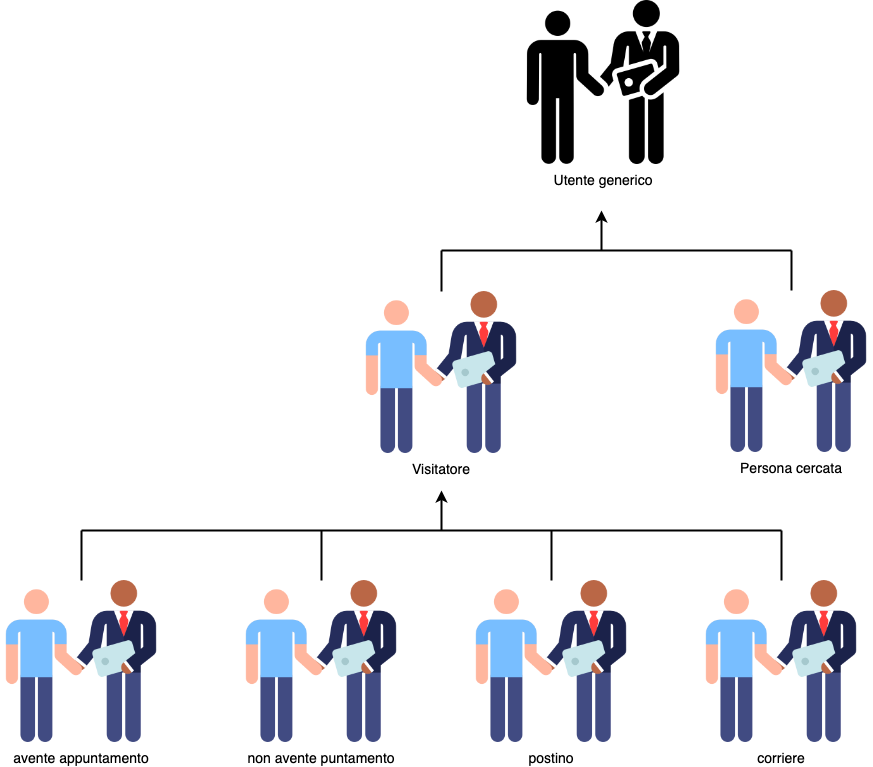
\includegraphics[width=0.8\columnwidth]{immagini/attori.png}
    \caption{\label{fig:attori}Utenti del sistema}
\end{figure}
\subsection{Casi d'uso - Visitatore}
Durante il periodo di tirocinio, la fase di analisi dei casi d'uso è da considerarsi divisa in due parti simili fra loro: quella dedicata al visitatore, ovvero colui che si presenta negli uffici dell'azienda avente un appuntamento registrato in calendario, o che semplicemente si presenta senza preavviso, e il servizio di consegna pacchi svolto dal postino o dal corriere. In entrambe le parti gli attori avvieranno la Skill installata nel dispositivo Amazon Echo Show e seguiranno le istruzioni riportate a voce dall'assistente vocale oppure mostrate a video dal display. In questa sezione viene riporta una rappresentazione grafica dei casi d'uso dell'utente identificato come "Visitatore avente appuntamento", che descrive le interazioni che l'attore svolge con il sistema. Di seguito viene riportato il diagramma dei casi d'uso individuati utilizzando lo standard UML 2.0
\begin{figure}[H] 
    \centering 
    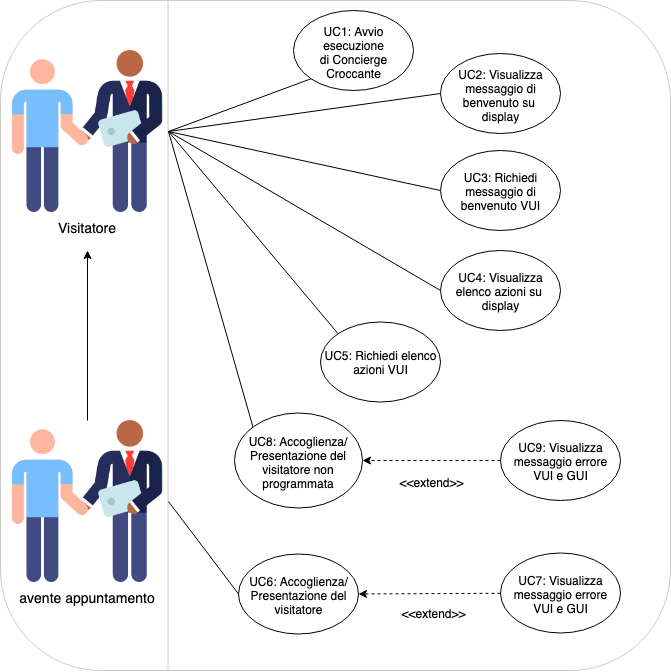
\includegraphics[width=1\columnwidth]{immagini/casi_duso1.png}
    \caption{\label{fig:casi_duso_visitatore}Casi d'uso visitatore avente appuntamento}
\end{figure}
Dall'elaborazione di tale analisi sono quindi emersi i seguenti casi d'uso riportati:
\begin{center}
	\centering
	\renewcommand{\arraystretch}{1.5}
	\rowcolors{3}{tableLight}{}
	\begin{longtable}{  p{2.5cm} p{9.8cm} }
		\rowcolor{tableHead}
		\textbf{\textcolor{white}{Identificativo}} & \textbf{\textcolor{white}{Descrizione}} \\
		\endhead  
		
		UC1 &  \textit{Attori}: visitatore avente o non avente appuntamento \newline \textit{Scopo}: l'utente può avviare Concierge Croccante \newline \textit{Pre-condizione}: il dispositivo Amazon deve aver avviato \mbox{l'assistente} Alexa \newline \textit{Post-condizione}: l'utente ha avviato Concierge Croccante \\
		
		UC2 &  \textit{Attori}: visitatore  \newline \textit{Scopo}: l'utente riceve un messaggio di benvenuto sul display del dispositivo \newline \textit{Pre-condizione}: la Skill Concierge Croccante deve essere stata avviata \newline \textit{Post-condizione}: l'utente riceve un messaggio di benvenuto sul display del dispositivo \\
		
		UC3 &  \textit{Attori}: visitatore  \newline \textit{Scopo}: l'utente riceve un messaggio vocale di benvenuto dalla Skill \mbox{Concierge} Croccante \newline \textit{Pre-condizione}: la Skill Concierge Croccante deve essere stata avviata \newline \textit{Post-condizione}: l'utente riceve un messaggio vocale dalla Skill Concierge Croccante\\
		
		UC4 &  \textit{Attori}: visitatore  \newline \textit{Scopo}: l'utente visualizza l'elenco sintetico ed essenziale di azioni sul \mbox{display} del dispositivo \newline \textit{Pre-condizione}: la Skill Concierge Croccante deve essere stata avviata \newline \textit{Post-condizione}: l'utente visualizza l'elenco di azioni sul display del dispositivo \\
		
		UC5 &  \textit{Attori}: visitatore  \newline \textit{Scopo}: viene esposto all'utente l'elenco sintetico ed essenziale di azioni \newline \textit{Pre-condizione}: la Skill Concierge Croccante deve essere stata avviata \newline \textit{Post-condizione}: viene esposto all'utente l'elenco di azioni disponibili da Concierge Croccante \\
		
		UC6 &  \textit{Attori}: visitatore avente appuntamento \newline \textit{Scopo}: l'utente può annunciarsi per essere accolto dalla persona cercata \newline \textit{Pre-condizione}: la Skill Concierge Croccante deve essere stata avviata \newline \textit{Post-condizione}: l'utente si annuncia \\
		
		UC7 &  \textit{Attori}: visitatore avente appuntamento \newline \textit{Scopo}: viene visualizzato un messaggio, su display e vocale, di errore specifico per l'eccezione riscontrata \newline \textit{Pre-condizione}: la Skill Concierge Croccante deve essere stata avviata \newline \textit{Post-condizione}: l'utente riceve un messaggio su display e vocale di errore\\
		
		UC8 &  \textit{Attori}: visitatore  \newline \textit{Scopo}: l'utente può annunciarsi per essere accolto dalla persona cercata \newline \textit{Pre-condizione}: la Skill Concierge Croccante deve essere stata avviata \newline \textit{Post-condizione}: l'utente si annuncia \\
		
		UC9 &  \textit{Attori}: visitatore  \newline \textit{Scopo}: viene visualizzato un messaggio, su display e vocale, di errore specifico per l'eccezione riscontrata \newline \textit{Pre-condizione}: la Skill Concierge Croccante deve essere stata avviata \newline \textit{Post-condizione}: l'utente riceve un messaggio su display e vocale di errore\\
		
		\rowcolor{white}
		\caption{\label{tab:UC_persona}Tabella casi d'uso visitatore avente appuntamento e non}
	\end{longtable}
\end{center}
\begin{figure}[H] 
    \centering 
    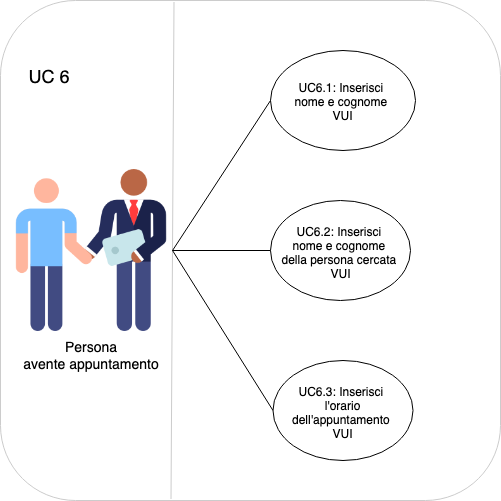
\includegraphics[width=0.7\columnwidth]{immagini/casi_duso2.png}
    \caption{\label{fig:sotto_casi_duso_visitatori1}Sotto casi d'uso visitatore avente appuntamento}
\end{figure}
\begin{center}
	\centering
	\renewcommand{\arraystretch}{1.5}
	\rowcolors{3}{tableLight}{}
	\begin{longtable}{  p{2.5cm} p{9.6cm} }
		\rowcolor{tableHead}
		\textbf{\textcolor{white}{Identificativo}} & \textbf{\textcolor{white}{Descrizione}} \\
		\endhead  
		
		UC6.1 &  \textit{Attori}: visitatore avente o non avente appuntamento \newline \textit{Scopo}: l'utente inserisce/dice il suo nome e cognome \newline \textit{Pre-condizione}: la Skill Concierge Croccante deve essere stata avviata \newline \textit{Post-condizione}: l'utente ha inserito/detto il suo nome e cognome \\
		
		UC6.2 &  \textit{Attori}: visitatore avente o non avente appuntamento \newline \textit{Scopo}: l'utente inserisce/dice il nome e cognome della persona che cerca \newline \textit{Pre-condizione}: la Skill Concierge Croccante deve essere stata avviata \newline \textit{Post-condizione}: l'utente ha inserito/detto il suo nome e cognome della persona cercata \\
		
		UC6.3 &  \textit{Attori}: visitatore avente o non avente appuntamento \newline \textit{Scopo}: l'utente inserisce/dice l'orario di appuntamento \newline \textit{Pre-condizione}: la Skill Concierge Croccante deve essere stata avviata \newline \textit{Post-condizione}: l'utente ha inserito/detto l'orario di appuntamento \\
		
		\rowcolor{white}
		\caption{Tabella sotto casi d'uso visitatore avente appuntamento e non}
	\end{longtable}
\end{center}
\begin{figure}[H] 
    \centering 
    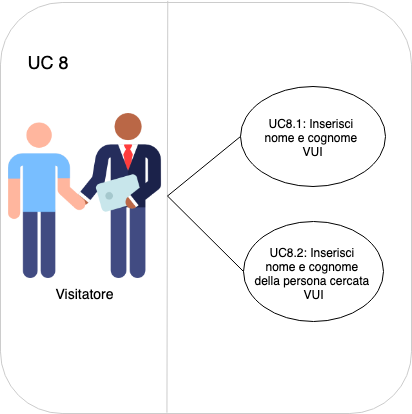
\includegraphics[width=0.7\columnwidth]{immagini/casi_duso21.png}
    \caption{\label{fig:sotto_casi_duso_visitatore2}Sotto casi d'uso visitatore avente appuntamento}
\end{figure}
\begin{center}
	\centering
	\renewcommand{\arraystretch}{1.5}
	\rowcolors{3}{tableLight}{}
	\begin{longtable}{  p{2.5cm} p{9.8cm} }
		\rowcolor{tableHead}
		\textbf{\textcolor{white}{Identificativo}} & \textbf{\textcolor{white}{Descrizione}} \\
		\endhead  
		
		UC8.1 &  \textit{Attori}: visitatore  \newline \textit{Scopo}: l'utente inserisce/dice il suo nome e cognome \newline \textit{Pre-condizione}: la Skill Concierge Croccante deve essere stata avviata \newline \textit{Post-condizione}: l'utente ha inserito/detto il suo nome e cognome \\
		
		UC8.2 &  \textit{Attori}: visitatore   \newline \textit{Scopo}: l'utente inserisce/dice il nome e cognome della persona che cerca \newline \textit{Pre-condizione}: la Skill Concierge Croccante deve essere stata avviata \newline \textit{Post-condizione}: l'utente ha inserito/detto il suo nome e cognome della persona cercata \\

		\rowcolor{white}
		\caption{Tabella sotto casi d'uso visitatore avente appuntamento e non}
	\end{longtable}
\end{center}
\subsection{Casi d'uso - Postino/Corriere}
La seconda parte di analisi dei casi d'uso, è dedicata al servizio di consegna dei pacchi che viene svolto dal postino o dal corriere. In questa sezione si rappresenta graficamente i casi d'uso dell'utente identificato come "Corriere", che descrive le interazioni che l'attore svolge con il sistema.
\\
\begin{figure}[H] 
    \centering 
    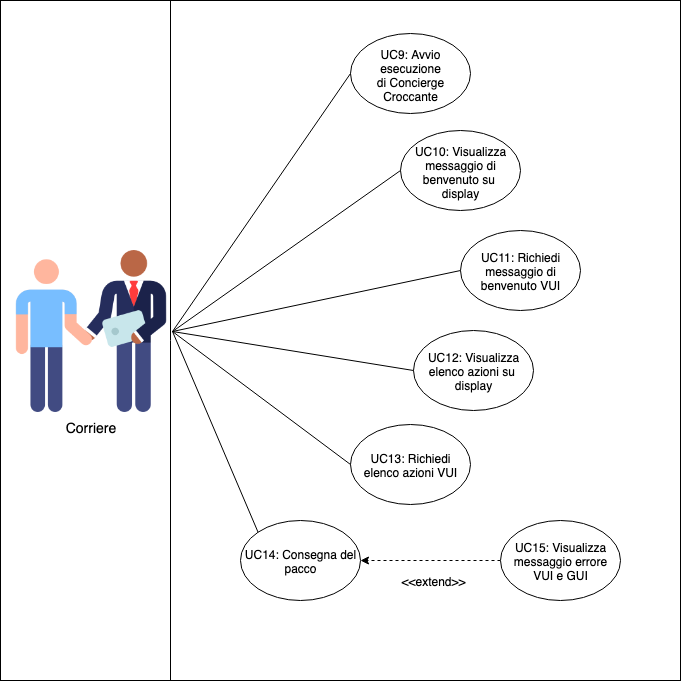
\includegraphics[width=1\columnwidth]{immagini/casi_duso3.png}
    \caption{\label{fig:casi_duso_corriere}Casi d'uso corriere}
\end{figure}
\newpage
\noindent Dall'elaborazione di tale analisi sono quindi emersi i seguenti casi d'uso riportati:
\begin{center}
	\centering
	\renewcommand{\arraystretch}{1.5}
	\rowcolors{3}{tableLight}{}
	\begin{longtable}{  p{2.5cm} p{9.8cm} }
		\rowcolor{tableHead}
		\textbf{\textcolor{white}{Identificativo}} & \textbf{\textcolor{white}{Descrizione}} \\
		\endhead  
		
		
		UC9 &  \textit{Attori}: corriere \newline \textit{Scopo}: l'utente può avviare Concierge Croccante \newline \textit{Pre-condizione}: il dispositivo Amazon deve aver avviato l'assistente Alexa \newline \textit{Post-condizione}: l'utente ha avviato Concierge Croccante \\
		
		UC10 &  \textit{Attori}: corriere \newline \textit{Scopo}: l'utente riceve un messaggio di benvenuto sul display del dispositivo \newline \textit{Pre-condizione}: la Skill Concierge Croccante deve essere stata avviata \newline \textit{Post-condizione}: l'utente riceve un messaggio di benvenuto sul display del dispositivo \\
		
		UC11 &  \textit{Attori}: corriere \newline \textit{Scopo}: l'utente riceve un messaggio vocale di benvenuto dalla Skill \mbox{Concierge} Croccante \newline \textit{Pre-condizione}: la Skill Concierge Croccante deve essere stata avviata \newline \textit{Post-condizione}: l'utente riceve un messaggio vocale dalla Skill C.C.\\
		
		UC12 &  \textit{Attori}: corriere \newline \textit{Scopo}: l'utente visualizza l'elenco sintetico ed essenziale di azioni sul \mbox{display} del dispositivo \newline \textit{Pre-condizione}: la Skill Concierge Croccante deve essere stata avviata \newline \textit{Post-condizione}: l'utente visualizza l'elenco di azioni sul display del dispositivo \\
		
		UC13 &  \textit{Attori}: corriere \newline \textit{Scopo}: viene esposto all'utente l'elenco sintetico ed essenziale di azioni \newline \textit{Pre-condizione}: la Skill Concierge Croccante deve essere stata avviata \newline \textit{Post-condizione}: viene esposto all'utente l'elenco di azioni disponibili da C.C. \\
		
		UC14 &  \textit{Attori}: corriere \newline \textit{Scopo}: l'utente può consegnare un pacco \newline \textit{Pre-condizione}: la Skill Concierge Croccante deve essere stata avviata \newline \textit{Post-condizione}: l'utente consegna il pacco \\
		
		UC15 &  \textit{Attori}: corriere \newline \textit{Scopo}: viene visualizzato un messaggio, su display e vocale, di errore specifico per l'eccezione riscontrata \newline \textit{Pre-condizione}: la Skill Concierge Croccante deve essere stata avviata \newline \textit{Post-condizione}: l'utente riceve un messaggio su display e vocale di errore\\
		
		UC17 &  \textit{Attori}: corriere \newline \textit{Scopo}: l'utente per consegnare il pacco richiede la presenza di una persona specifica per una firma \newline \textit{Pre-condizione}: la Skill Concierge Croccante deve essere stata avviata \newline \textit{Post-condizione}: l'utente riceve la firma desiderata e consegna il pacco\\
		
		UC18 &  \textit{Attori}: corriere \newline \textit{Scopo}: l'utente per consegnare il pacco richiede la presenza di una persona per una firma \newline \textit{Pre-condizione}: la Skill Concierge Croccante deve essere stata avviata \newline \textit{Post-condizione}: l'utente riceve la firma desiderata e consegna il pacco\\
		\rowcolor{white}
		\caption{Tabella casi d'uso corriere}
	\end{longtable}
\end{center}

\newpage
\section{Voice User Interface - VUI}
\label{vui}
Altro aspetto importante dell'analisi è stata sulla Voice User Interface, che nel documento verrà abbreviato con l'acronimo VUI. La VUI per la Skill è l’interfaccia che rende possibile l’interazione umana parlata con il computer, utilizzando il riconoscimento vocale per comprendere comandi e domande vocali, ed infine il text to speech per riprodurre una risposta. Nel caso del progetto la VUI è rappresentata dall'assistente vocale Amazon Alexa, la quale eseguirà la Skill prodotta. Vista la ovvia complessità che presenta un'interazione umana vocale con un computer, la VUI fornita dall'assistente vocale Alexa presenta alcuni limiti che verranno analizzati successivamente in un nuovo punto del capitolo.\\
L’obbiettivo che si prefigge nel realizzare la Skill è quello di poter sostenere una conversazione, il più naturale possibile, con la persona accolta all'entrata dell'azienda Crispy Bacon. L’idea è quindi che l’ospite possa dialogare con Concierge Croccante, motivare la presenza in azienda e notificare l’interessato della visita. Dall'analisi emerge una conversazione come l'esempio seguente in formato testo di quello che si vuole ottenere dal prodotto finale:
\begin{figure}[H] 
    \centering 
    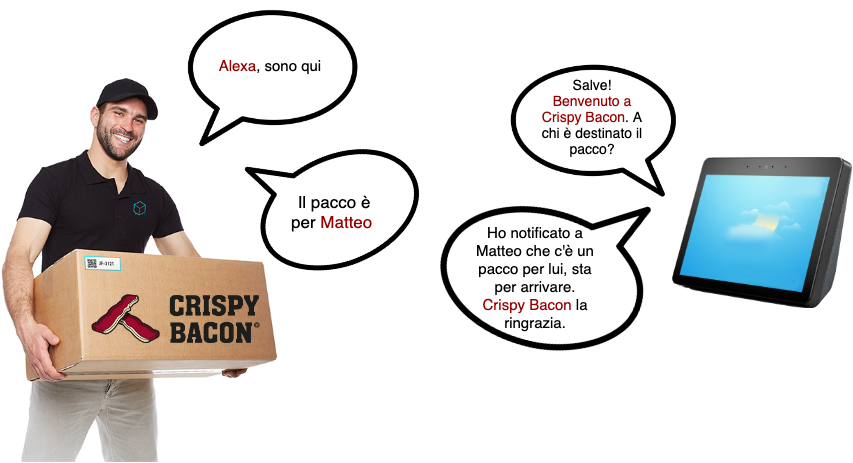
\includegraphics[width=1\columnwidth]{immagini/esempioVUI.png}
    \caption{\label{fig:esempioVUI}Esempio di conversazione}
\end{figure}
\begin{itemize}
	\item \textbf{Utente}: \textit{"Alexa, sono qui."}
	\item \textbf{Concierge}: \textit{ "Buongiorno! Benvenuto a Crispy Bacon, quale è il motivo della sua visita?"}
	\item \textbf{Utente}: \textit{"Devo consegnare un pacco."}
	\item \textbf{Concierge}: \textit{ "Chi è il destinatario del pacco?"}
	\item \textbf{Utente}: \textit{"Matteo P."}
	\item \textbf{Concierge}: \textit{ "Ho notificato a Matteo che c'è un pacco per lui, sta per arrivare."}
	\item \textbf{Concierge}: \textit{ "Crispy Bacon la ringrazia."}
\end{itemize}
La Skill Concierge Croccante necessita quindi di ricevere dati in input per poter completare il processo di accoglienza della persona entrata in azienda. È quindi necessario suddividere i dati richiesti in base alla tipo di utente:
\begin{center}
	\centering
	\renewcommand{\arraystretch}{1.5}
	\rowcolors{3}{tableLight}{}
	\begin{longtable}{  p{4.5cm} p{8.3cm} }
		\rowcolor{tableHead}
		\textbf{\textcolor{white}{Tipo di utente}} & \textbf{\textcolor{white}{Dati da raccogliere}} \\
		\endhead  
		
		Persona senza \mbox{appuntamento} &  - Proprio nome \newline - Proprio cognome \newline - Nome persona cercata  \newline - Cognome persona cercata \\
		Persona con \mbox{appuntamento} &  - Proprio nome \newline - Proprio cognome \newline - Nome persona cercata  \newline - Cognome persona cercata \newline - Orario dell'appuntamento \\
		Corriere &  - Il proprio titolo (corriere) \newline - Nome della persona interessata \newline - Cognome della persona interessata \\
		Postino &  - Il proprio titolo (postino) \newline - Nome della persona interessata \newline - Cognome della persona interessata \\
		\rowcolor{white}
		\caption{Tabella tipologia dati per tipo di utente}
	\end{longtable}
\end{center}
\subsection{Voice Flow}
Al termine della fase di analisi sulla VUI si ha ottenuto come risultato il Voice Flow, ovvero il percorso ipotetico che l’utente può intraprendere durante la conversazione con la Skill Concierge Croccante, rappresentato dal diagramma di attività secondo lo standard UML 2.0. Quest'ultimo è un tipo di diagramma che permette la descrizione un processo attraverso dei grafi in cui i nodi rappresentano le attività e gli archi l'ordine con cui vengono eseguite. Permette inoltre la descrivere gli aspetti dinamici dei casi d'uso e supporta l'elaborazione parallela.
\begin{figure}[H] 
    \centering 
    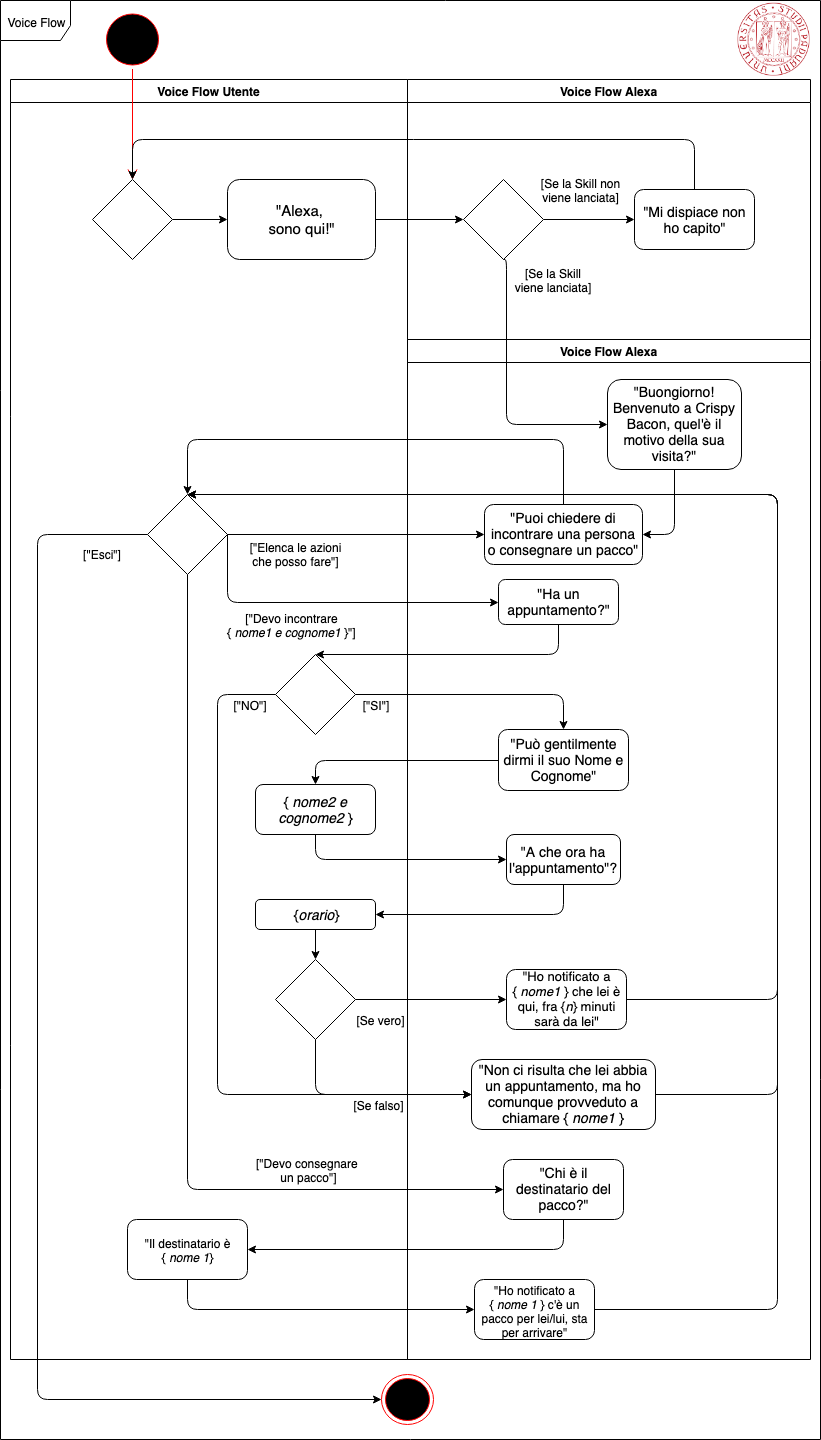
\includegraphics[width=1\columnwidth]{immagini/attivita.png}
    \caption{\label{fig:voice_flow}Diagramma di attività VUI - Concierge Croccante}
\end{figure}
\subsection{Interazione vocale - UC6}
Di seguito si riporta l'analisi descrittiva e testuale dell'interazione vocale del UC6, riportato in tabella ?, considerato significativo per la comprensione dei dialoghi.
\begin{itemize}
	\item \textit{Utente - Visitatore}: "Salve! Devo incontrare \texttt{\{nome1 e cognome1\}}."
	\item[-] \textit{Alexa - Concierge Croccante}:  "Può gentilmente dirmi il suo nome e cognome?" 
	\item \textit{Utente - Visitatore}: "\texttt{\{nome2 e cognome2\}}."
	\item[-] \textit{Alexa - Concierge Croccante}:  "A che ora ha l'appuntamento?"
	\item \textit{Utente - Visitatore}: "\texttt{\{orario\}}."
	\item[-] \textit{Alexa - Concierge Croccante}:  "Ho notificato a \texttt{\{nome1\}} che lei è qui, fra pochi secondi sarà da lei."
\end{itemize}
Altra casistica:
\begin{itemize}
	\item \textit{Utente - Visitatore}: "Salve! Sono \texttt{\{nome2 e cognome2\}}, devo incontrare \texttt{\{nome1 e cognome1\}}."
	\item[-] \textit{Alexa - Concierge Croccante}:  "Ha un appuntamento?"
	\item \textit{Utente - Visitatore}: "Si."
	\item[-] \textit{Alexa - Concierge Croccante}:  "A che ora ha l'appuntamento?"
	\item \textit{Utente - Visitatore}: "\texttt{\{orario\}}."
	\item[-] \textit{Alexa - Concierge Croccante}:  "Ho notificato a \texttt{\{nome1\}} che lei è qui, fra pochi secondi sarà da lei."
\end{itemize}
Nel caso in cui l'utente non abbia un appuntamento o non risulta nel calendario l'incontro, si riceverà la seguente risposta: 
\begin{itemize}
	\item[-] \textit{Alexa - Concierge Croccante}:  "Non ci risulta che lei abbia un appuntamento, ma ho comunque provveduto a chiamare \texttt{\{nome1\}}."
\end{itemize}
\newpage
\section{Graphical User Interface - GUI}
Un altro aspetto, studiato per concludere tutti gli aspetti dell'analisi, è stata la Graphical User Interface, che nel documento verrà abbreviato con l'acronimo GUI. La GUI è l'interfaccia grafica utente che consente l’interazione uomo-macchina in modo visuale utilizzando rappresentazioni grafiche. Nel caso del progetto la GUI è costituita da delle Multimodal Displays, ovvero delle visuals che riportano dei dati (anche linkati) e delle funzionalità, mostrate sullo schermo del dispositivo Amazon Echo Show. Le visuals mostrate sono quindi a supporto della VUI e hanno il compito di riportare a video informazioni utili a migliorare la conversazione uomo-macchina.
\\
\begin{figure}[H] 
    \centering 
    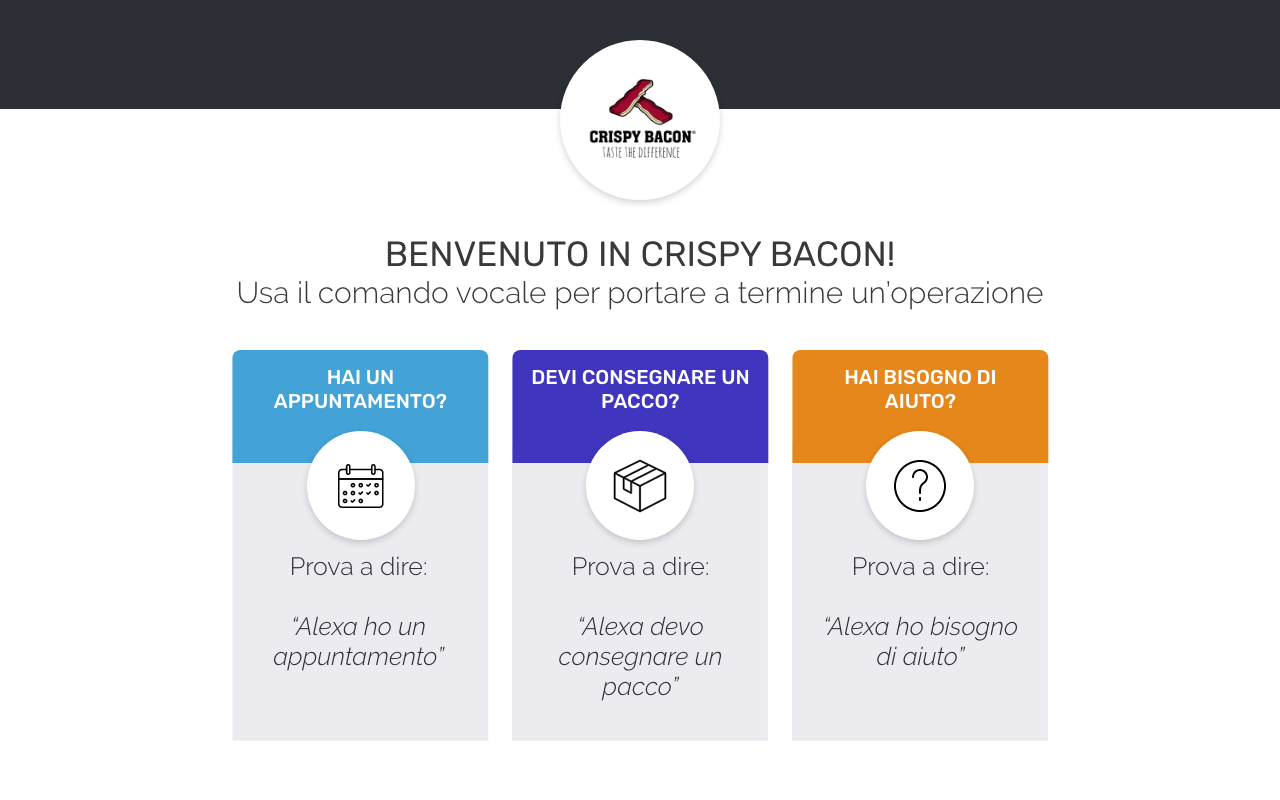
\includegraphics[width=1\columnwidth]{immagini/home_gui.jpg}
    \caption{\label{fig:esempioGUI}Esempio GUI - Home}
\end{figure}
\newpage
\noindent La GUI svolge quindi il compito di supporto per aiutare e migliorare l’esperienza di dialogo. L’immagine sopra riporta una visual che propone di presentare dei dati secondo quel determinato layout. In questa fase di analisi vengono esposti alcuni layout significativi che mostrano a schermo alcune informazioni:
\\[0.4cm]
\begin{minipage}{0.47\textwidth}
	\begin{figure}[H]
		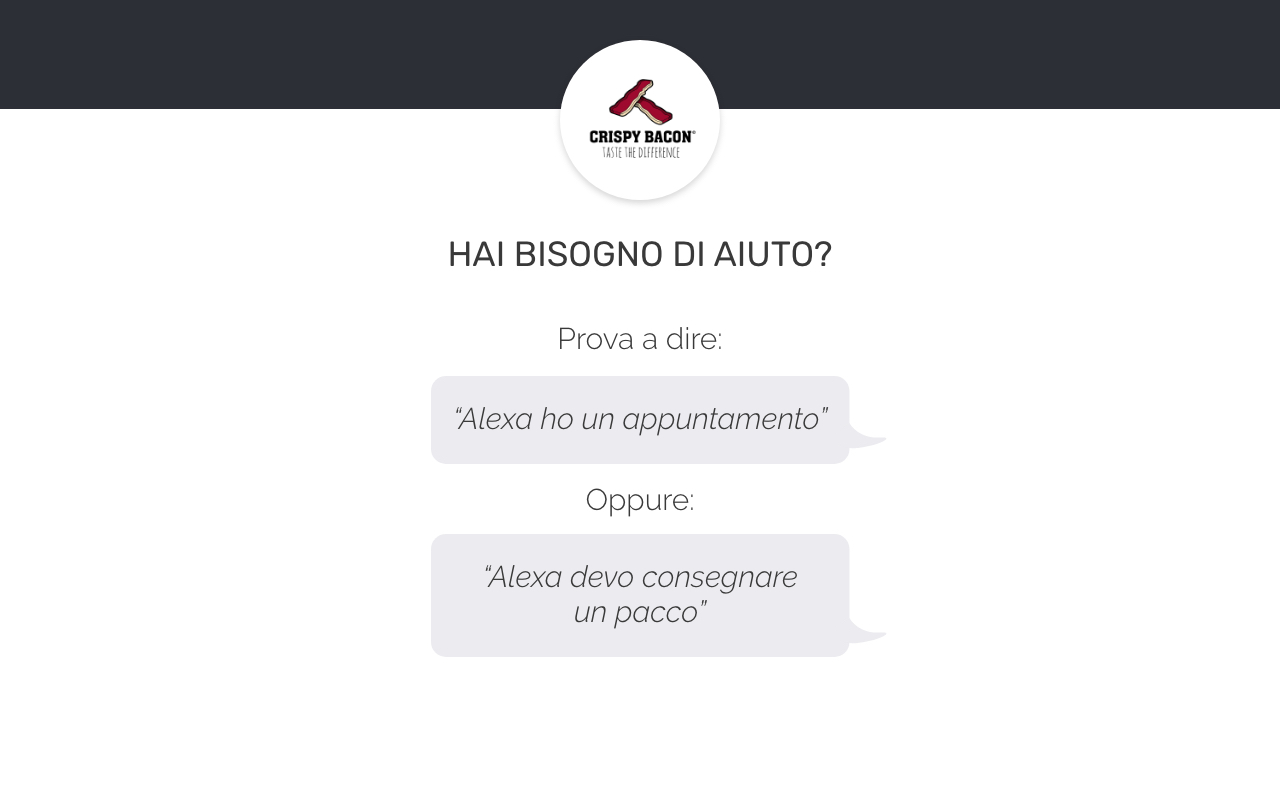
\includegraphics[width=1\columnwidth]{immagini/aiuto_gui.jpg}
		\caption{\label{fig:esempioGUI2}Esempio di visual - Aiuto}
	\end{figure}
\end{minipage}
\begin{minipage}{0.5\textwidth}
	\begin{itemize}  
		\item Titolo - \texttt{Nome dell'azienda}
		\item Azione \texttt{n}
		\item Immagine azione \texttt{n}
		\item \textit{altre informazioni}
	\end{itemize}
\end{minipage}
\\[0.4cm]
\begin{minipage}{0.47\textwidth}
	\begin{figure}[H]
		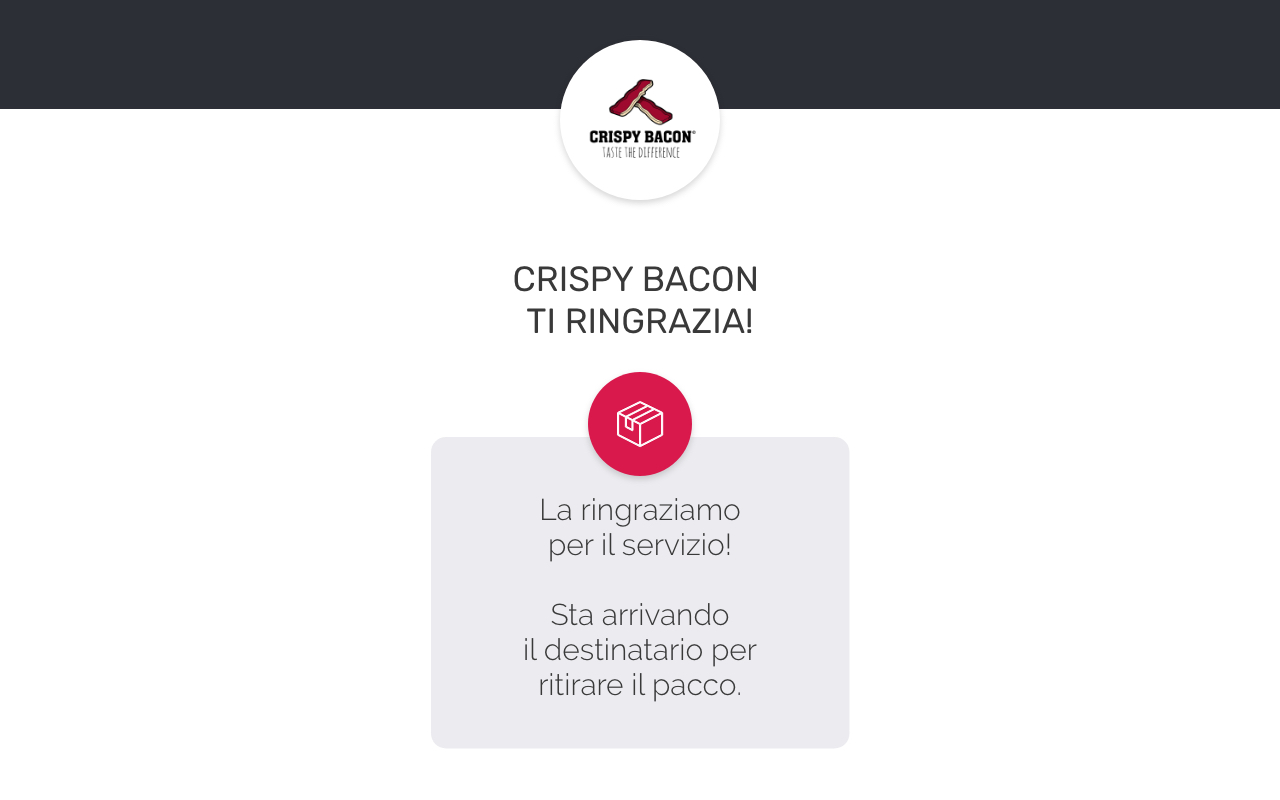
\includegraphics[width=1\columnwidth]{immagini/consegna_gui.jpg}
		\caption{\label{fig:esempioGUI3}Esempio di visual - Consegna}
	\end{figure}
\end{minipage}
\begin{minipage}{0.5\textwidth}
	\begin{itemize}  
		\item Titolo - \texttt{Nome dell'azienda}
		\item Informazione
		\item Immagine allegata
		\item \textit{altre informazioni}
	\end{itemize}
\end{minipage}
\\[0.4cm]
\begin{minipage}{0.47\textwidth}
	\begin{figure}[H]
		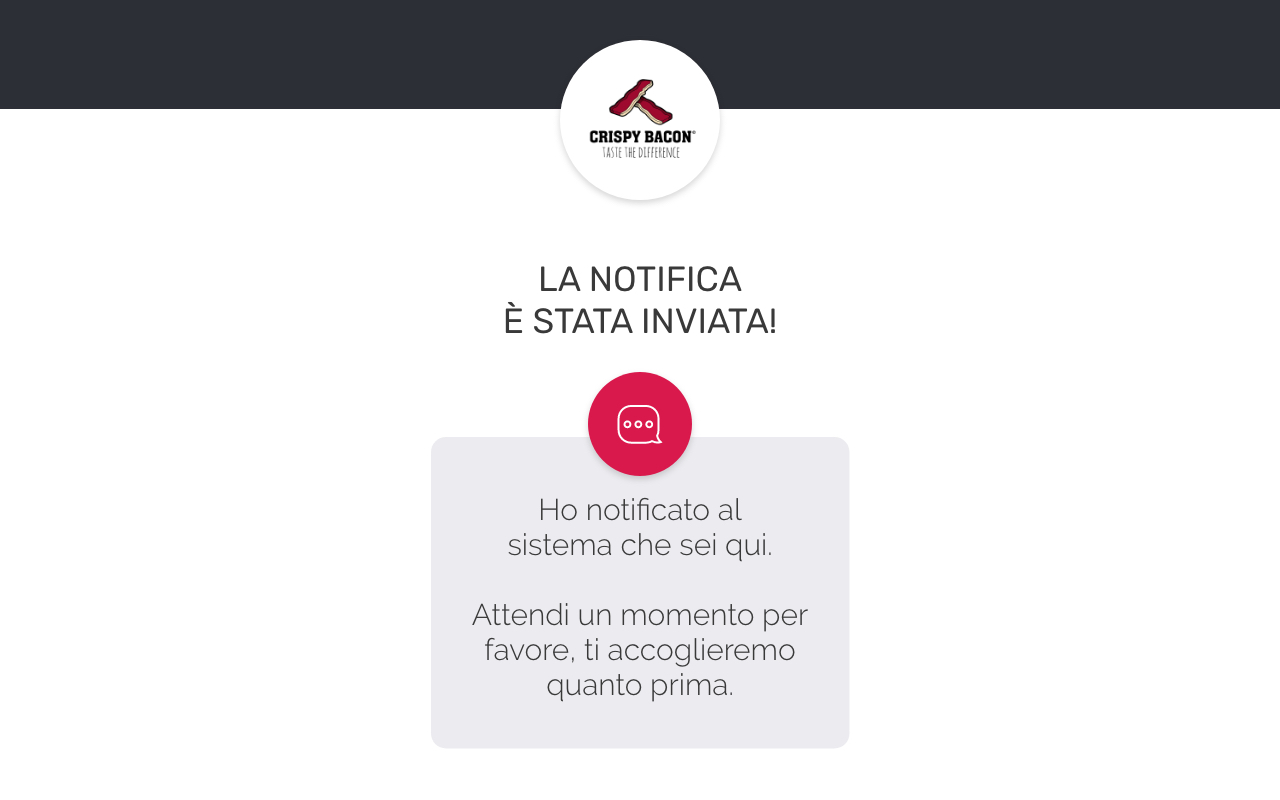
\includegraphics[width=1\columnwidth]{immagini/incontri_gui.jpg}
		\caption{\label{fig:esempioGUI4}Esempio di visual - Visitatore avente appuntamento}
	\end{figure}
\end{minipage}
\begin{minipage}{0.5\textwidth}
	\begin{itemize}  
		\item Titolo - \texttt{Nome dell'azienda}
		\item Informazioni sull'appuntamento
		\item Immagine allegata
		\item \textit{altre informazioni}
	\end{itemize}
\end{minipage}

\newpage
\section{Limiti}
Come già in precedenza menzionato gli assistenti vocali presentano dei limiti, in quanto non riescono a sostenere una conversazione completamente naturale con una persona umana. Nel contesto del progetto i limiti che si riscontrano nella Skill e Alexa sono i seguenti:
\begin{itemize}
	\item Alexa
	\begin{itemize}
		\item Non è possibile richiamare l'attenzione dell'assistente vocale senza pronunciare la parola \textit{"Alexa"};
		\item Per motivi linguistici l'assistente vocale può fare fatica a comprendere i nomi di persone;
	\end{itemize}
	\item Skill Concierge Croccante
	\begin{itemize}
		\item La Skill non può essere avviata senza il lancio da parte di Alexa;
		\item La Skill, per motivi implementativi, non può rimanere in ascolto per più di 8 secondi in attesa di una risposta da parte dell'utente.
	\end{itemize}
\end{itemize}